\chapter{直感的にツリーを作成できるインターフェース}
先行研究である「ゴオルシェア」では,システムを直感的に操作することが難しかった.
本研究では,初めて使う人でも直感的に操作できるインターフェースを目指した.

\section{画面構成}
本システムの画面構成を,スクリーンキャプチャと共に以下に示す.

\subsection{ミッション一覧}
作成されたミッション一覧を閲覧できる画面を\ref{img:interface_capture_list}に示す.
ミッションはカード型に,タイトルと作成者を閲覧することができる.

\begin{figure}[t]
	\begin{center}
		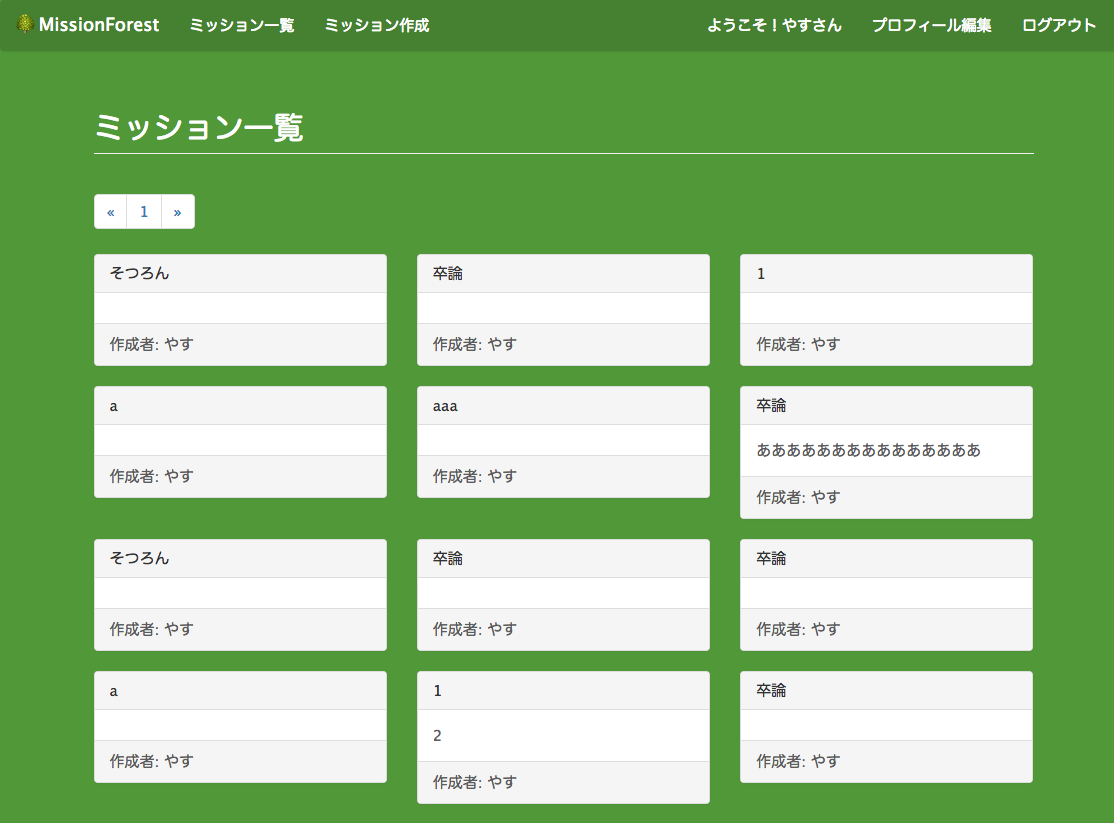
\includegraphics[width=0.9\linewidth]{assets/img/interface_capture_list.png}
		\caption{動作画面}
		\label{img:interface_capture_list}
	\end{center}
\end{figure}

\subsection{ミッション詳細}
ミッションの詳細画面を\ref{img:interface_capture_detail}に示す.
ミッションのタイトル,作成者,概要とともに,ミッションツリーを閲覧することができる.

\begin{figure}[t]
	\begin{center}
		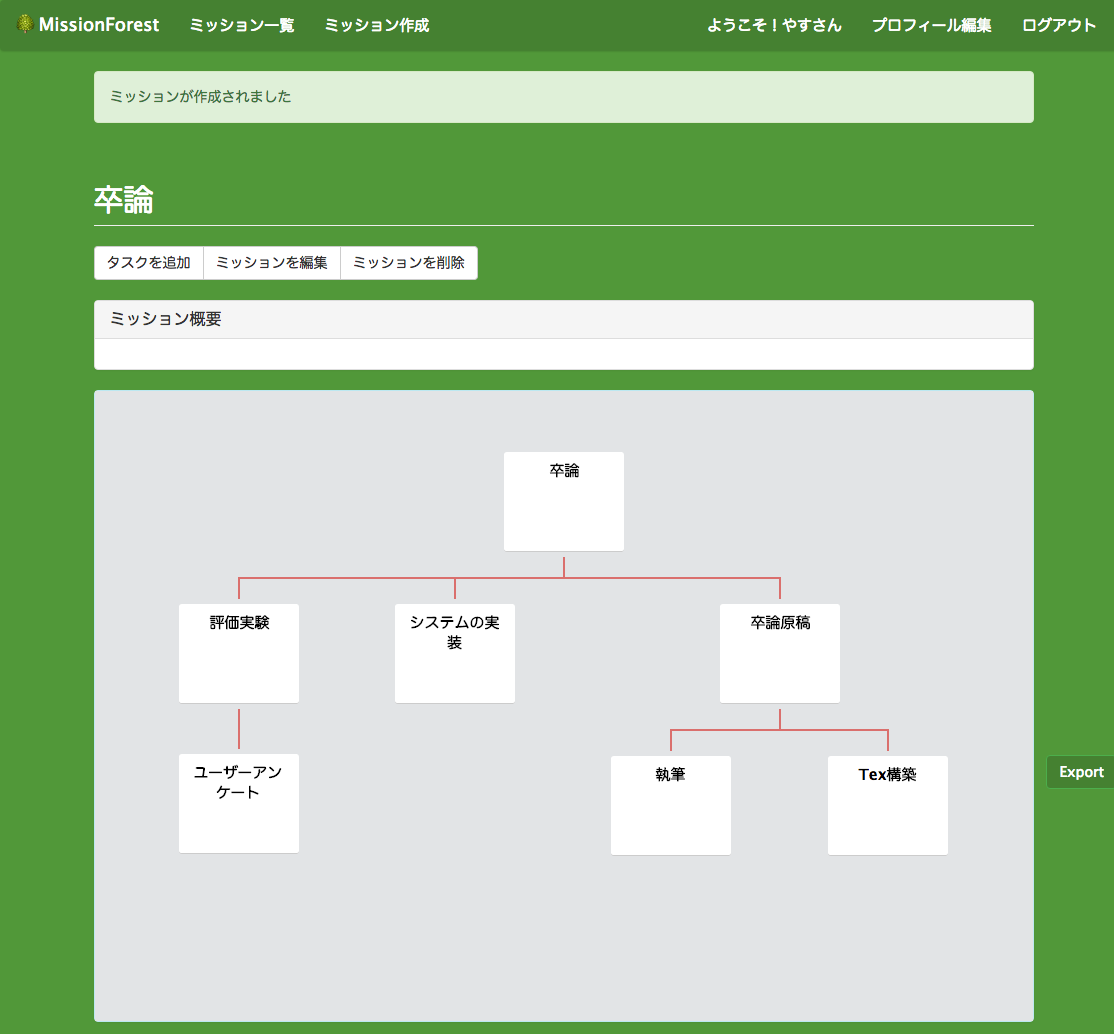
\includegraphics[width=0.9\linewidth]{assets/img/interface_capture_detail.png}
		\caption{動作画面}
		\label{img:interface_capture_detail}
	\end{center}
\end{figure}

\subsection{タスク追加}
タスクの追加画面を\ref{img:interface_capture_add}に示す.
タスクをクリックするとその子タスクを追加するモーダルが表示され,タスク名,概要,締め切りを入力することができる.

\begin{figure}[t]
	\begin{center}
		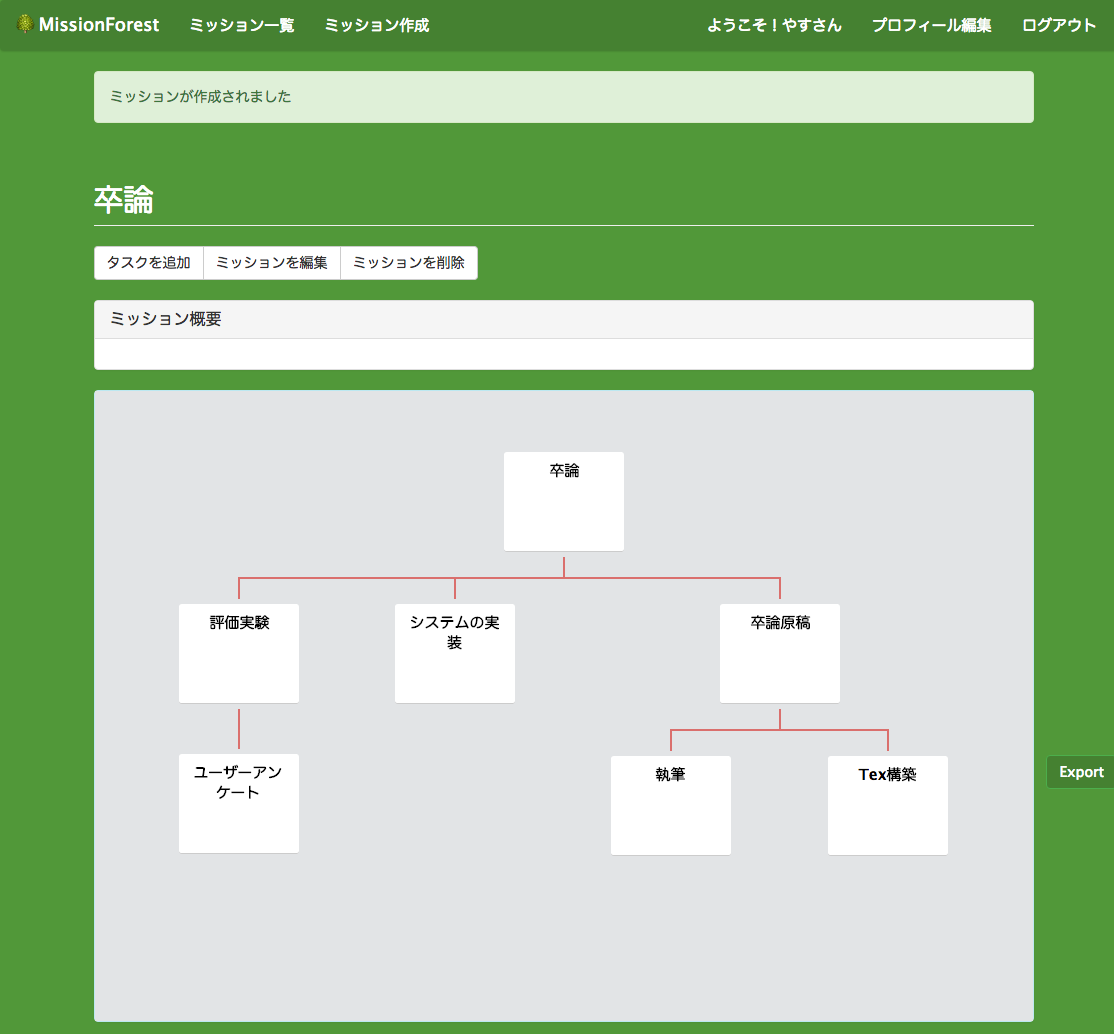
\includegraphics[width=0.9\linewidth]{assets/img/interface_capture_add.png}
		\caption{動作画面}
		\label{img:interface_capture_add}
	\end{center}
\end{figure}

\section{アプリケーション}
\subsection{Ajaxによる非同期通信}
従来のシステムでは,タスクを追加するたびにページ読み込みが発生し,1つのミッションを完成させるのに時間がかかっていた.
またページ読み込みされてしまうので,自分がどのタスクを編集していたのかが分かりづらかった.
そこで,本システムではAjaxを用いた非同期通信を用いることで,ページ読み込みなしにタスク追加をすることができるようにした.
また,サーバーとの通信は適切なデータのみをJSON形式でやり取りするので,レスポンスも向上した.

\subsection{システム構成}
本システムのシステム構成を図\ref{img:system_architecture}に示す.
まずプロジェクトを閲覧する場合,Webブラウザから非同期通信によってWebAPIにアクセスする.
WebAPIはメインデータベースであるMySQLからユーザー認証情報,ミッションやタスクの情報を取得し,JSON形式でレスポンスを返す.
次にプロジェクトを投稿する場合,Webブラウザから非同期通信によってWebAPIにJSON形式でデータをPOSTし,WebAPIはメインデータベースであるMySQLに受け取ったデータを保存する.
さらに,タスクごとに設定されたアクセス権限によって,RDFストアであるStardogにLODとして保存する.

\begin{figure}[t]
	\begin{center}
		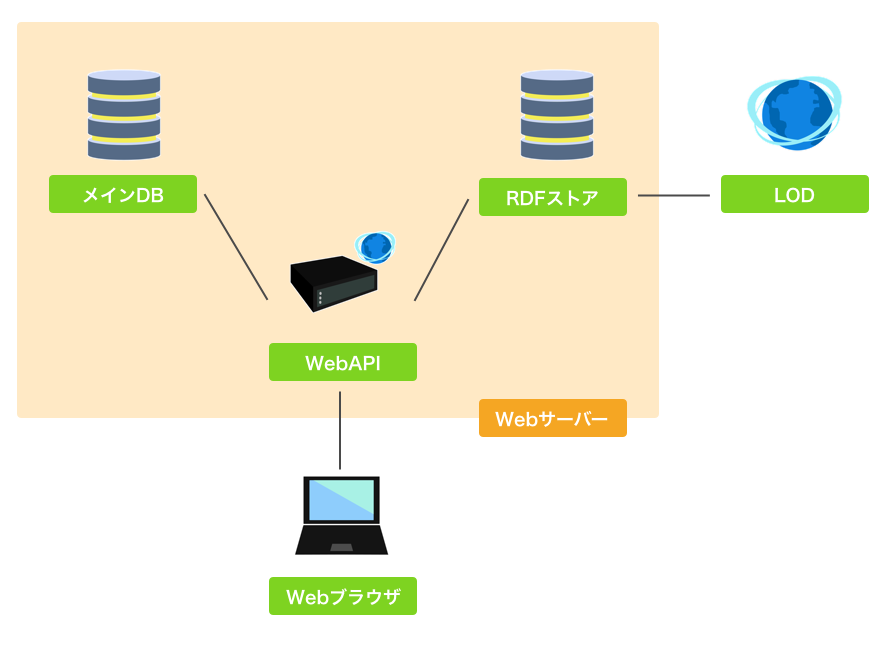
\includegraphics[width=0.9\linewidth]{assets/img/system_architecture.png}
		\caption{システム構成図}
		\label{img:system_architecture}
	\end{center}
\end{figure}

\section{主な機能}
試作するシステムでは,プロジェクトを「ミッション」と呼ぶ.
ユーザーは任意にミッションを作成することができ,ミッションごとに直感的なGUIでタスクツリーを構築することができる.
タスクには進捗状況の指定,タグの指定,コメント機能,編集履歴,ファイル添付をすることができる.
作成したミッションは任意のタイミングで一般公開することができるので,公開されたミッション間から後述するアルゴリズム類似ミッションを推定し,ユーザーに推薦することにより,組織を越えた協働を促進する.

\section{ツリーエディタ}
直感的なツリーエディタGUIを作成するため,本研究で使用したJavaScriptライブラリを述べる.

\subsection{実装手法}
dabengが開発したOrgChart\footnote{https://github.com/dabeng/OrgChart}というjQueryライブラリをベースに拡張し,ミッションツリーを表現している.
このOrgChartでは,タスクのレイアウトに,HTMLのテーブル機能を用いている.
具体的には,HTMLのテーブル属性(<table>)は,カラム(<td>)の要素数に応じて列の幅が均等にレイアウトされる.
この性質を用い,1階層を1テーブルとみなし,テーブルのカラムの中にテーブルをネストすることで,HTMLにより再帰的にすべてのカラムが等間隔に配置される.

また先ほど述べたように,Ajaxを用いた非同期通信をするために,ツリーに表示するデータはAPIから\ref{img:json_sample}に示すようなJSON形式で取得している.
タスクの追加,編集,削除があった場合は,このデータとなるJSONが変更されるので,ツリーエディタ上も変更される.

\begin{figure}[t]
	\begin{center}
		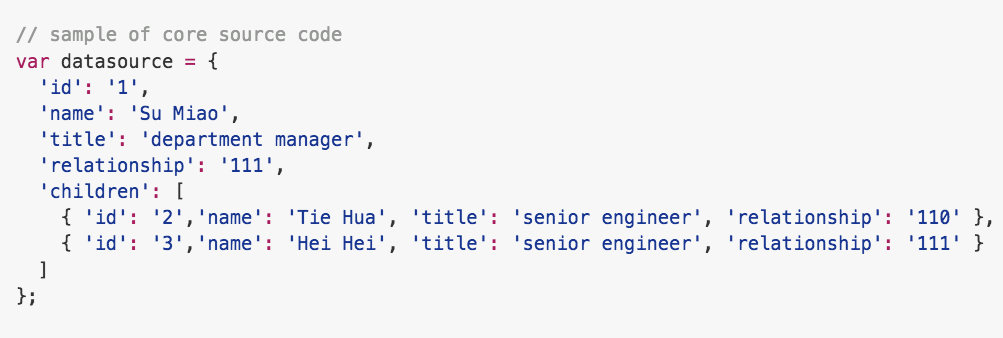
\includegraphics[width=0.9\linewidth]{assets/img/json_sample.png}
		\caption{システム構成図}
		\label{img:json_sample}
	\end{center}
\end{figure}
